% 第 2 周交付物:特征工程说明文档 v2(中文版) —— 编译方式:XeLaTeX
% v2(2026-07-28,应导师意见修订):补全每个特征的含义与选择原因;新增相关性与重要性分析章节
\documentclass[11pt]{ctexart}
\usepackage[a4paper, margin=2.4cm]{geometry}
\usepackage{amsmath}
\usepackage{booktabs}
\usepackage{graphicx}
\usepackage[hidelinks]{hyperref}
\usepackage{enumitem}
\setlist{nosep}

\title{\textbf{特征工程说明文档(v2)}\\
\large Advanced Chooser Option Pricing Model --- 第 2 周交付物}
\author{佟铸城 (Zhucheng Tong)}
\date{2026 年 7 月(v2 修订:补充特征释义与相关性/重要性分析)}

\begin{document}
\maketitle

\section{清洗决策}
管道入口:\texttt{python -m src.preprocess},输出至 \texttt{data/processed/}。

\begin{center}
\small
\begin{tabular}{p{3.2cm} p{4.6cm} p{6.0cm}}
\toprule
\textbf{步骤} & \textbf{决策} & \textbf{理由} \\
\midrule
日历对齐 & 全部序列重索引到 NYSE 交易日历(JPM 的 1760 个交易日) & JPM 期权在此日历上交易;宏观序列不应引入幽灵行 \\
FRED 节假日缺口 & 日频序列(国债收益率、利差)做时间线性插值 & 利率变动缓慢,时间插值是标准且无偏的做法 \\
FEDFUNDS(月频) & 前向填充(阶梯函数) & 政策利率在两次 FOMC 之间保持不变,插值会凭空制造政策变动 \\
离群值(IQR, $k=3$) & \textbf{标记但保留},审计记录存 \texttt{outlier\_report.json} & 被标记的极值日全部对应真实市场事件(最极端:2020-03 COVID 崩盘)。删除它们等于抹掉本项目第 4 周要研究的高波动区间 \\
\bottomrule
\end{tabular}
\end{center}

\section{特征释义:含义、计算与选择原因}
共 18 个特征(任务要求 $\geq 10$),按经济含义分五组。每个特征按\textbf{含义 / 计算 / 选择原因}三要素说明。

\subsection{收益与已实现波动率(5 个)}
\begin{enumerate}
  \item \texttt{log\_return} --- \textbf{含义}:JPM 日对数收益率。\textbf{计算}:$\ln(P^{adj}_t/P^{adj}_{t-1})$(复权价)。\textbf{选择原因}:一切波动率估计的原材料;对数收益可跨期加总,是定价模型的标准输入形式。
  \item \texttt{realized\_vol\_21d / 63d / 252d} --- \textbf{含义}:过去 1 个月/1 个季度/1 年的年化已实现波动率。\textbf{计算}:对应窗口对数收益标准差 $\times\sqrt{252}$。\textbf{选择原因}:BSM 的 $\sigma$ 输入的直接候选;三个窗口刻画波动率期限结构——短窗口反应快但噪声大,长窗口平滑但滞后。同时纳入是为了让 ML 模型自行学习"该听哪个窗口的",这正是 BSM 常数波动率假设做不到的;
  \item \texttt{parkinson\_vol\_21d} --- \textbf{含义}:基于日内高低价极差的月度波动率。\textbf{计算}:$\sqrt{\frac{1}{4\ln 2}\,\overline{[\ln(H/L)]^2}}\times\sqrt{252}$。\textbf{选择原因}:只用收盘价会丢掉日内信息;Parkinson 估计量利用高低价,统计效率约为收盘价法的 5 倍,在剧烈波动但收盘变动不大的日子(如 2020-03)提供增量信号。
\end{enumerate}

\subsection{股息(2 个)}
\begin{enumerate}
  \setcounter{enumi}{5}
  \item \texttt{div\_yield\_ttm} --- \textbf{含义}:滚动 12 个月股息率。\textbf{计算}:过去 252 交易日股息合计 / 不复权收盘价。\textbf{选择原因}:即 BSM 公式中的 $q$;chooser 的 put--call parity 分解显式依赖 $q$,必须精确;
  \item \texttt{div\_growth\_yoy} --- \textbf{含义}:TTM 股息的同比增速。\textbf{计算}:TTM 股息合计的 252 日同比变化率。\textbf{选择原因}:任务书指定的股息动态特征;股息增速变化往往对应公司基本面/资本政策的状态切换,为 ML 提供慢变量背景。
\end{enumerate}

\subsection{利率(4 个)}
\begin{enumerate}
  \setcounter{enumi}{7}
  \item \texttt{r\_3m / r\_1y} --- \textbf{含义}:3 个月/1 年期国债收益率(小数)。\textbf{计算}:FRED DGS3MO、DGS1 $/100$。\textbf{选择原因}:BSM 的无风险利率 $r$;chooser 有两个期限($t_1=0.5$ 与 $T_2=1$),分别需要匹配期限的贴现率;
  \item \texttt{curve\_slope} --- \textbf{含义}:收益率曲线斜率(10 年 $-$ 2 年利差)。\textbf{计算}:FRED T10Y2Y。\textbf{选择原因}:曲线倒挂是经典的衰退/风险状态信号,为波动率状态切换提供宏观领先信息;
  \item \texttt{rate\_momentum\_21d} --- \textbf{含义}:长端利率一个月内的变化幅度。\textbf{计算}:DGS10 的 21 日差分。\textbf{选择原因}:任务书指定的利率动量;2022 年式的快速加息期本身就是高波动状态,该特征将"利率变化的速度"显式喂给模型。
\end{enumerate}

\subsection{市场背景(3 个)}
\begin{enumerate}
  \setcounter{enumi}{11}
  \item \texttt{spx\_log\_return} --- \textbf{含义}:标普 500 日对数收益。\textbf{计算}:同 \texttt{log\_return},标的换为 \^{}GSPC。\textbf{选择原因}:市场因子;JPM 作为系统重要性银行,其波动很大程度由大盘驱动;
  \item \texttt{beta\_63d} --- \textbf{含义}:JPM 对大盘的滚动贝塔。\textbf{计算}:63 日窗口 $\mathrm{cov}(r_{JPM},r_{SPX})/\mathrm{var}(r_{SPX})$。\textbf{选择原因}:分离系统性与个股特质波动;贝塔的时变本身是风险状态的刻画(全样本均值 0.93,量级合理);
  \item \texttt{corr\_jpm\_vix\_63d} --- \textbf{含义}:JPM 收益与 VIX 变动的滚动相关。\textbf{计算}:63 日窗口 $\mathrm{corr}(r_{JPM},\Delta \mathrm{VIX})$。\textbf{选择原因}:任务书指定;该相关通常为负(杠杆效应),其强弱变化标记市场"恐慌传导"的松紧。
\end{enumerate}

\subsection{情绪(4 个,全部由 VIX 派生;经导师确认以 VIX 替代新闻数据)}
\begin{enumerate}
  \setcounter{enumi}{14}
  \item \texttt{vix\_level} --- \textbf{含义}:VIX 收盘价,市场对未来 30 天的隐含波动率预期。\textbf{计算}:\^{}VIX 原始水平。\textbf{选择原因}:VIX 由标普 500 期权价格反解,是唯一\textbf{前瞻性}的波动率信息(其余 realized vol 均为回望);含方差风险溢价,即市场为对冲恐慌支付的价格;
  \item \texttt{vix\_sentiment\_pct} --- \textbf{含义}:VIX 在过去一年中所处的分位位置,即任务书要求的 \textbf{0--1 情绪分}。\textbf{计算}:VIX 的滚动 252 日百分位。\textbf{选择原因}:把 VIX 的绝对水平转换为\textbf{相对状态}(同样是 VIX=20,在平静年份是高位、在动荡年份是低位),百分位天然归一到 $[0,1]$ 且对状态切换敏感;
  \item \texttt{vix\_momentum\_5d} --- \textbf{含义}:VIX 一周内的变化量,情绪切换速度。\textbf{计算}:VIX 的 5 日差分。\textbf{选择原因}:恐慌上升期与消退期对波动率的含义不同(骤升往往伴随波动率聚集的开始),动量项让模型区分"高位企稳"与"急速拉升";
  \item \texttt{fear\_regime} --- \textbf{含义}:恐慌状态哑变量。\textbf{计算}:情绪百分位 $>0.75$ 或 VIX $>30$ 时置 1。\textbf{选择原因}:为线性模型和最终定价工具提供可解释的状态开关;也用于第 4 周按状态分组的 BSM 失效分析。
\end{enumerate}

\textbf{VIX 双重角色的控制}:原始水平只承担波动率角色,情绪角色仅由标准化变换承担;VIX 反映大盘而非 JPM 个股情绪,为已知局限。

\section{相关性分析}
对模型可用集(1289 行,截至 2024-11,剔除目标缺失尾部)计算 18 特征的 Pearson 相关矩阵,见图~\ref{fig:corr}。

\begin{figure}[h!]
\centering
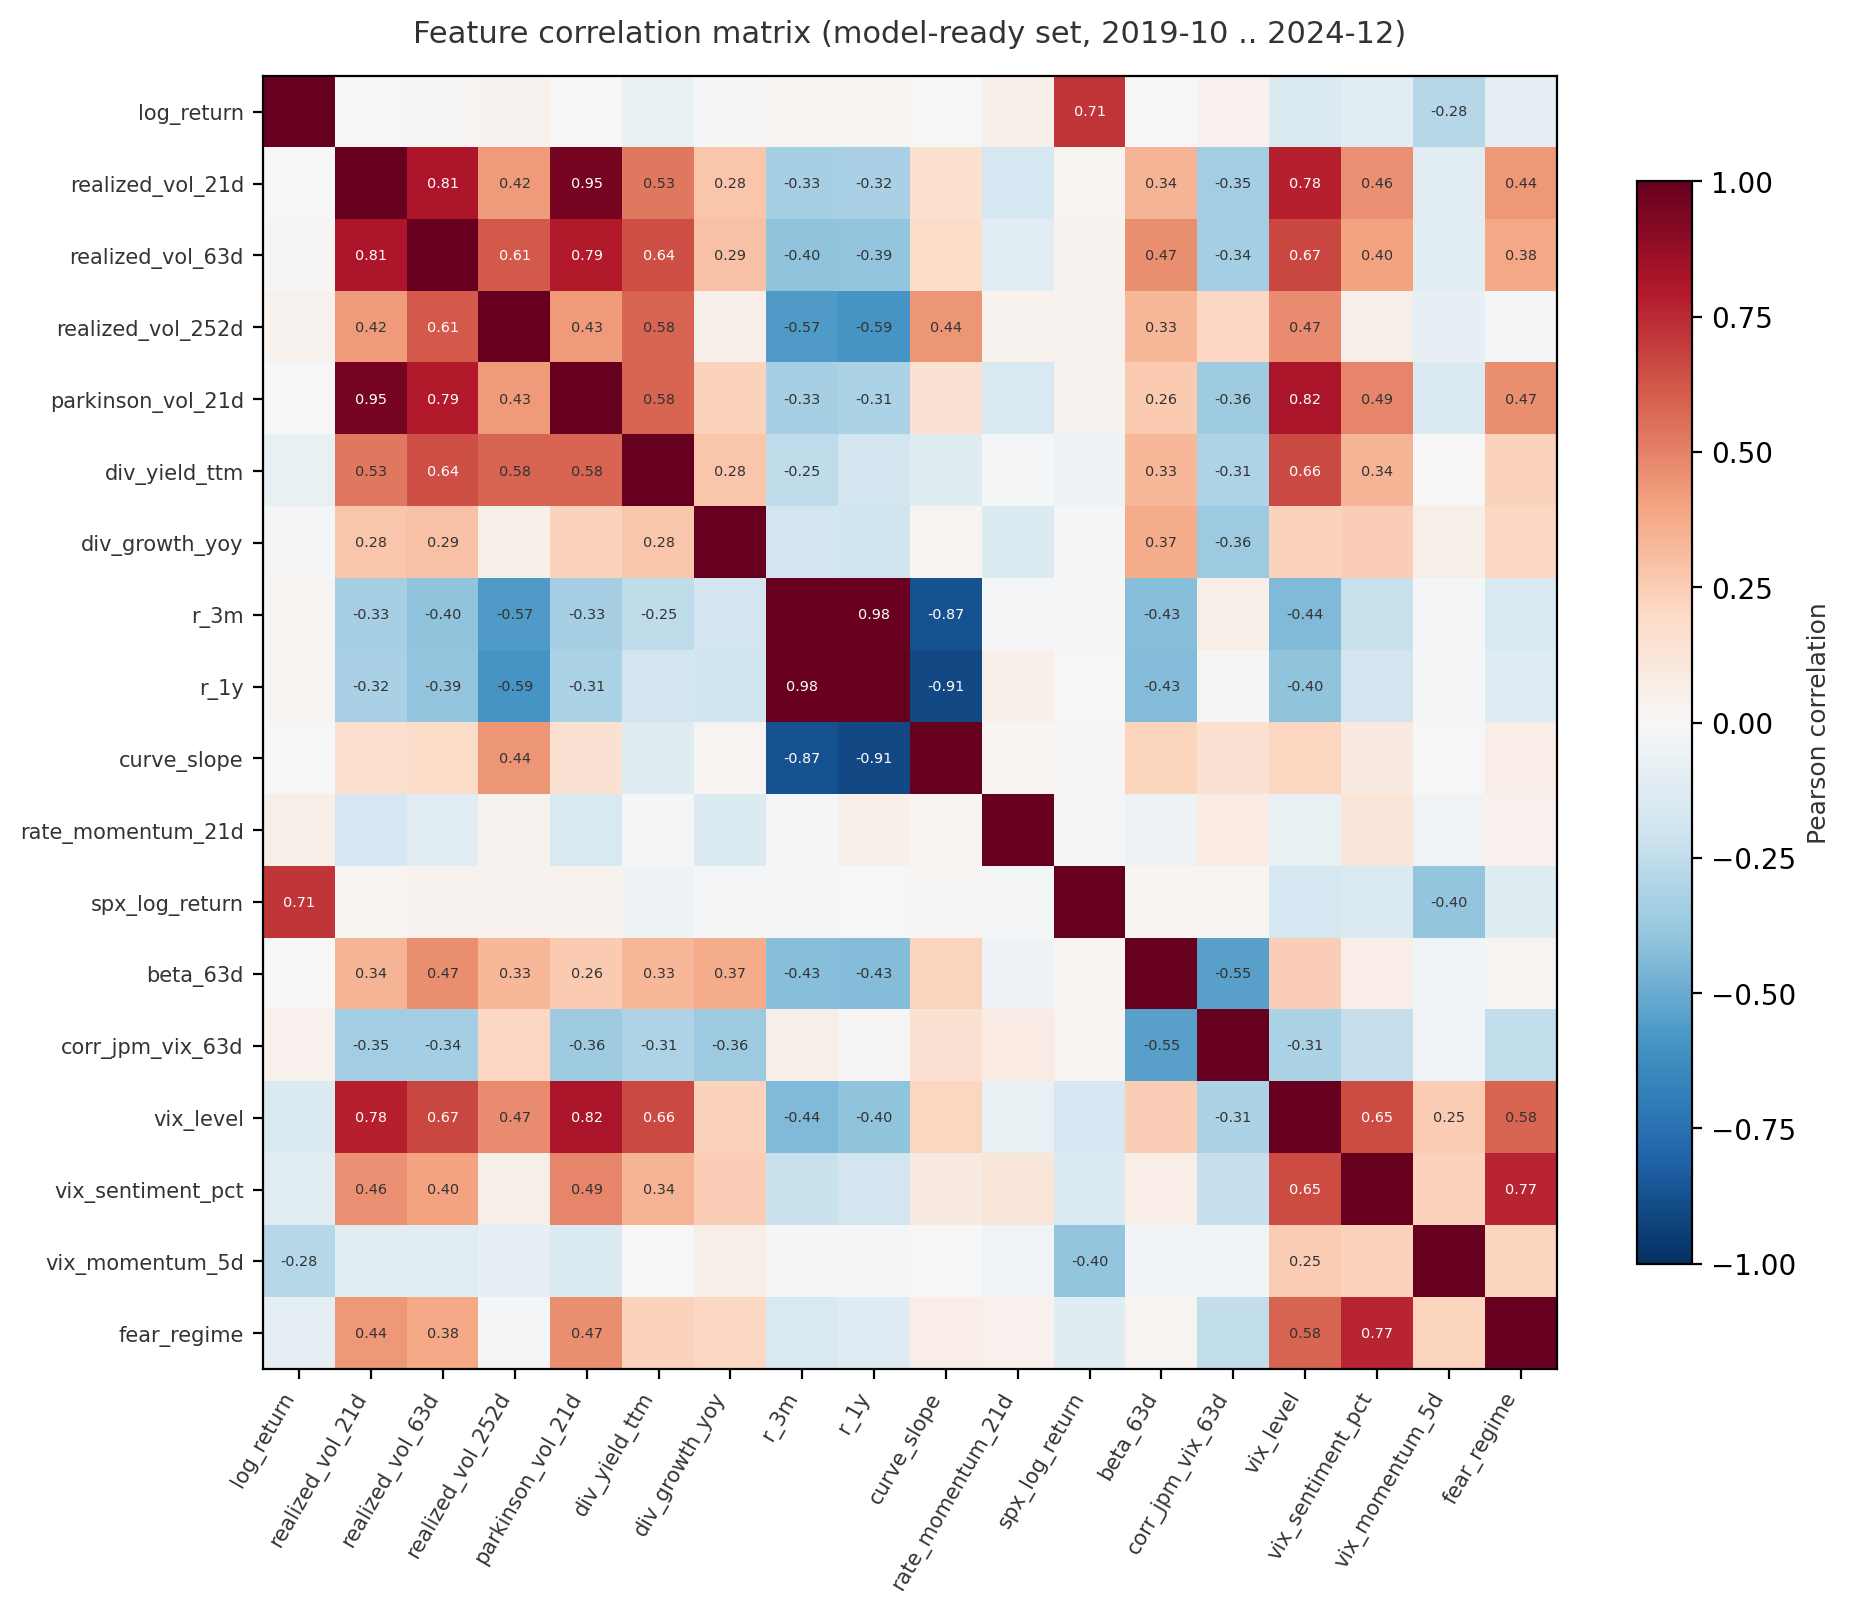
\includegraphics[width=0.92\textwidth]{figures/corr_heatmap.png}
\caption{特征相关性矩阵(仅标注 $|r|\geq 0.25$ 的单元格)}
\label{fig:corr}
\end{figure}

三个结构性发现:
\begin{enumerate}
  \item \textbf{利率块}:\texttt{r\_3m} 与 \texttt{r\_1y} 相关 $+0.98$,二者与 \texttt{curve\_slope} 相关 $-0.87/-0.91$——样本期内(2022--2023 加息周期)短端快速抬升导致曲线走平/倒挂,符合宏观事实。建模含义:线性模型不应同时纳入两条短端利率,W5 的线性基线将只保留期限匹配的 \texttt{r\_1y} 或做正则化;
  \item \textbf{波动率块}:五个波动率特征互相关 $0.78$--$0.95$(最高为 \texttt{realized\_vol\_21d}$\sim$\texttt{parkinson\_vol\_21d} 的 $+0.95$)。这是预期中的共线——它们度量同一对象的不同侧面;树模型对此不敏感,线性模型需降维或选代表;
  \item \textbf{情绪块与波动率块的联结}:\texttt{vix\_level} 与已实现波动率相关 $0.78$--$0.82$,但 \texttt{vix\_sentiment\_pct}(百分位变换后)与之相关降至 $0.40$--$0.49$——说明标准化确实剥离了一部分水平信息、保留了状态信息,双重角色的控制有效。
\end{enumerate}

\section{重要性分析}
以\textbf{未来 21 日已实现波动率}为目标变量(第 5 周 ML 路线 A 的预测对象),用两种独立口径评估特征重要性:随机森林不纯度重要性(捕捉非线性与交互)与互信息(无模型的单变量依赖),见图~\ref{fig:imp}。

\begin{figure}[h!]
\centering
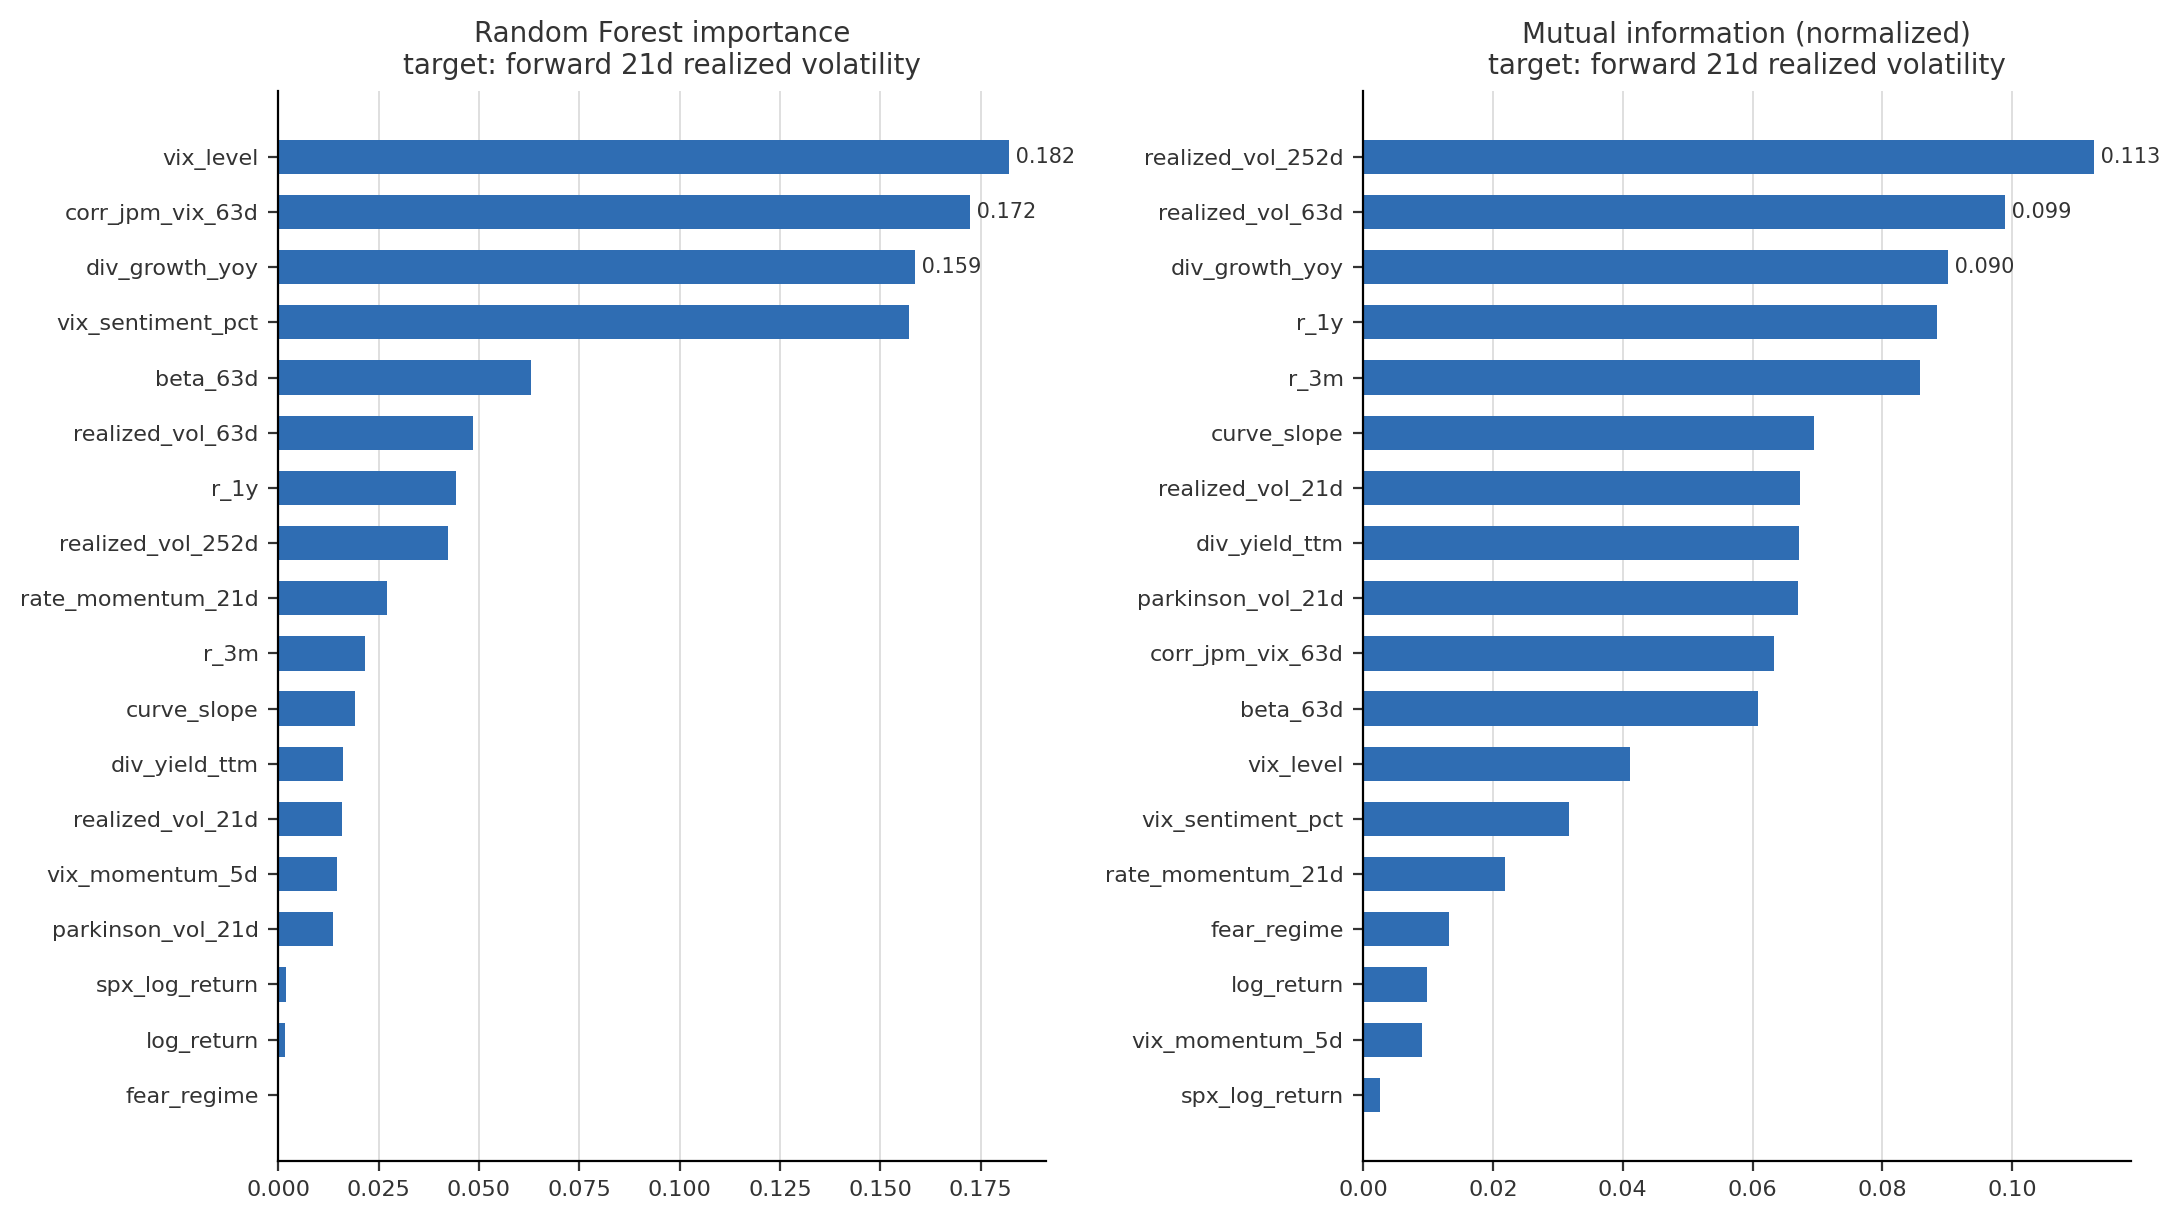
\includegraphics[width=\textwidth]{figures/feature_importance.png}
\caption{特征重要性:随机森林(左)与互信息(右),目标为前瞻 21 日已实现波动率}
\label{fig:imp}
\end{figure}

\begin{enumerate}
  \item \textbf{RF 口径的头部特征}:\texttt{vix\_level}(0.182)、\texttt{corr\_jpm\_vix\_63d}(0.172)、\texttt{div\_growth\_yoy}(0.159)、\texttt{vix\_sentiment\_pct}(0.157)。与目标的单变量相关也是 \texttt{vix\_level} 最高($|r|=0.62$)。\textbf{前瞻性的 VIX 系特征整体压过回望性的已实现波动率},与方差风险溢价文献(隐含波动率是未来已实现波动率的有偏但信息量最大的预测量)一致——这为第 5 周"用含 VIX 的特征集预测波动率、再喂给 BSM"的路线提供了直接的数据背书;
  \item \textbf{两口径的分歧本身有信息}:互信息口径下长窗口已实现波动率(\texttt{realized\_vol\_252d}: 0.113)最高——单变量看,波动率的长记忆是最稳的依赖;而 RF 在多变量条件结构下更看重 VIX 系特征——说明 VIX 的\textbf{增量}信息主要体现在与其他特征的交互中。两口径都不低的 \texttt{div\_growth\_yoy} 需谨慎解读:更可能是"股息政策变动期恰逢波动状态切换"的代理效应而非因果,W6 将用 SHAP 进一步检验;
  \item \textbf{\texttt{fear\_regime} 在 RF 口径重要性 $\approx 0$}:其信息已被连续版的 \texttt{vix\_sentiment\_pct} 吸收(两者相关 $+0.77$)。保留它的理由是可解释性与定价工具的状态展示,而非预测增量——这一点在文档中如实说明;
  \item \textbf{方法论提示}:本节重要性为\textbf{探索性}分析(全样本拟合,未做时序切分),用于指导特征取舍;第 5--6 周的正式训练与评估将采用 70/15/15 时序切分以杜绝前视偏差。
\end{enumerate}

\section{输出、验证与自动化}
数据集:全历史 1760 行;模型可用集 1309 行零缺失(2019-10-17 至 2024-12-30),CSV/Parquet 双格式;离群值审计 \texttt{outlier\_report.json}。合理性抽检:21 日已实现波动率均值 26.9\%(与论文 $\sigma=28.2\%$ 印证);2020-03-16 行(收益 $-16.2\%$、VIX 82.7、情绪百分位 1.0、恐慌标记 1)自洽。自动化:GitHub Actions 每周五收盘后执行采集$\to$预处理$\to$提交,已在云端实跑成功;分析脚本 \texttt{python -m src.analysis\_w2} 可一键复现本文档全部图表。

\end{document}
